\part{Os cantos do homem-sombra}

\chapter*{}
\thispagestyle{empty}

\vspace*{\fill}
\textit{Os Hupd'äh contam muitas histórias sobre pessoas que, andando pela mata, se
encontraram com seres da gente-sombra. Os homens e mulheres-sombra são muito fortes e perigosos. Eles usam várias roupas de cores diferentes para caçar e fazer mal às pessoas hup. Uma dessas roupas tem cor de sombra, daí o seu nome. A gente-sombra causa doenças e pode matar e comer a carne e o espírito das pessoas humanas. Mas muitos deles são sábios, e conhecem cantos, mitos e benzimentos. Esta é a história do encontro de um homem hup com um homem-sombra chamado Way Naku.}
\vspace*{\fill}

\openany

\chapter*{}
\mbox{}\vspace*{\fill}

\begingroup\raggedright\setlength{\linewidth}{.6\linewidth}


\letra{N}{o} alto de uma árvore de
cucura, um homem-sombra
chamado Way Naku cantava
um \textit{caapivaiá}.

\vspace{2em}

\letra{B}{atɨ̗b’} mah yup, Way Naku
batɨ̗b’ mah yup pö̗h yamah,
pɨ̗g tëganah.

\vspace*{\fill}

\pagebreak

\begin{textblock*}{8in}(0pt,0pt)%
\vspace*{-2.8cm}
\hspace*{-3.2cm}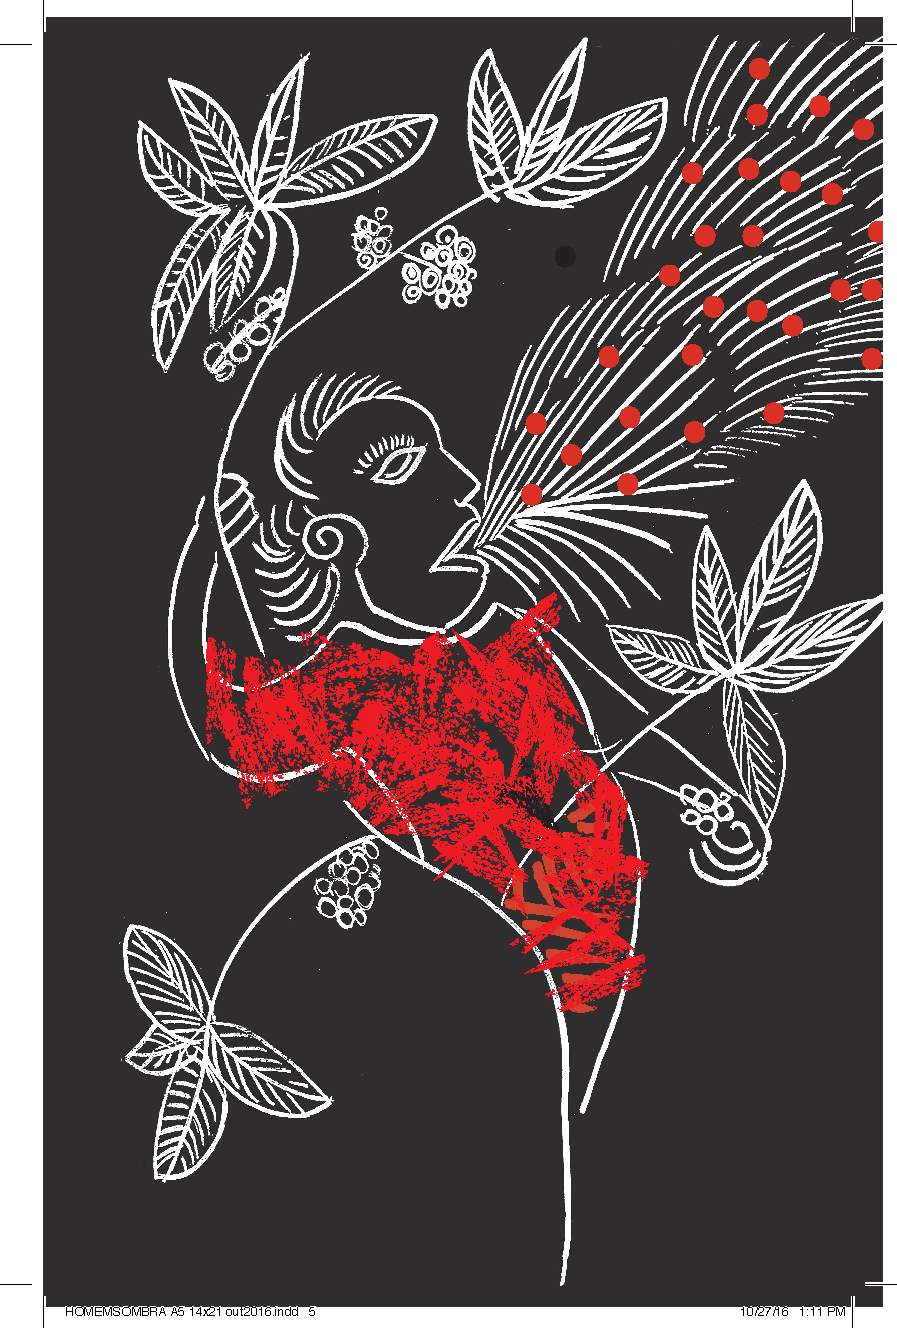
\includegraphics[width=153mm]{./imgs/img1.pdf}
\end{textblock*}

\chapter*{}

\mbox{}\vspace*{\fill}

\letra{E}{ncantado} com a música,
um homem hup aproximou-se,
sentou-se ao pé da
árvore e ficou escutando as
canções do homem-sombra. O
homem hup estava sentado,
pescando no igarapé
enquanto ouvia a música.

\vspace{2em}

\letra{P}{ɨ̗g} tëgan tɨh yam mɨ’ mah,
hup tɨh mɨ’ wɨ’ pemeh, tú.
Dë̖h máh hõ̖p käk pemep ɨhɨh.

\vspace*{\fill}

\pagebreak

\begin{textblock*}{8in}(0pt,0pt)%
\vspace*{-2.8cm}
\hspace*{-3.2cm}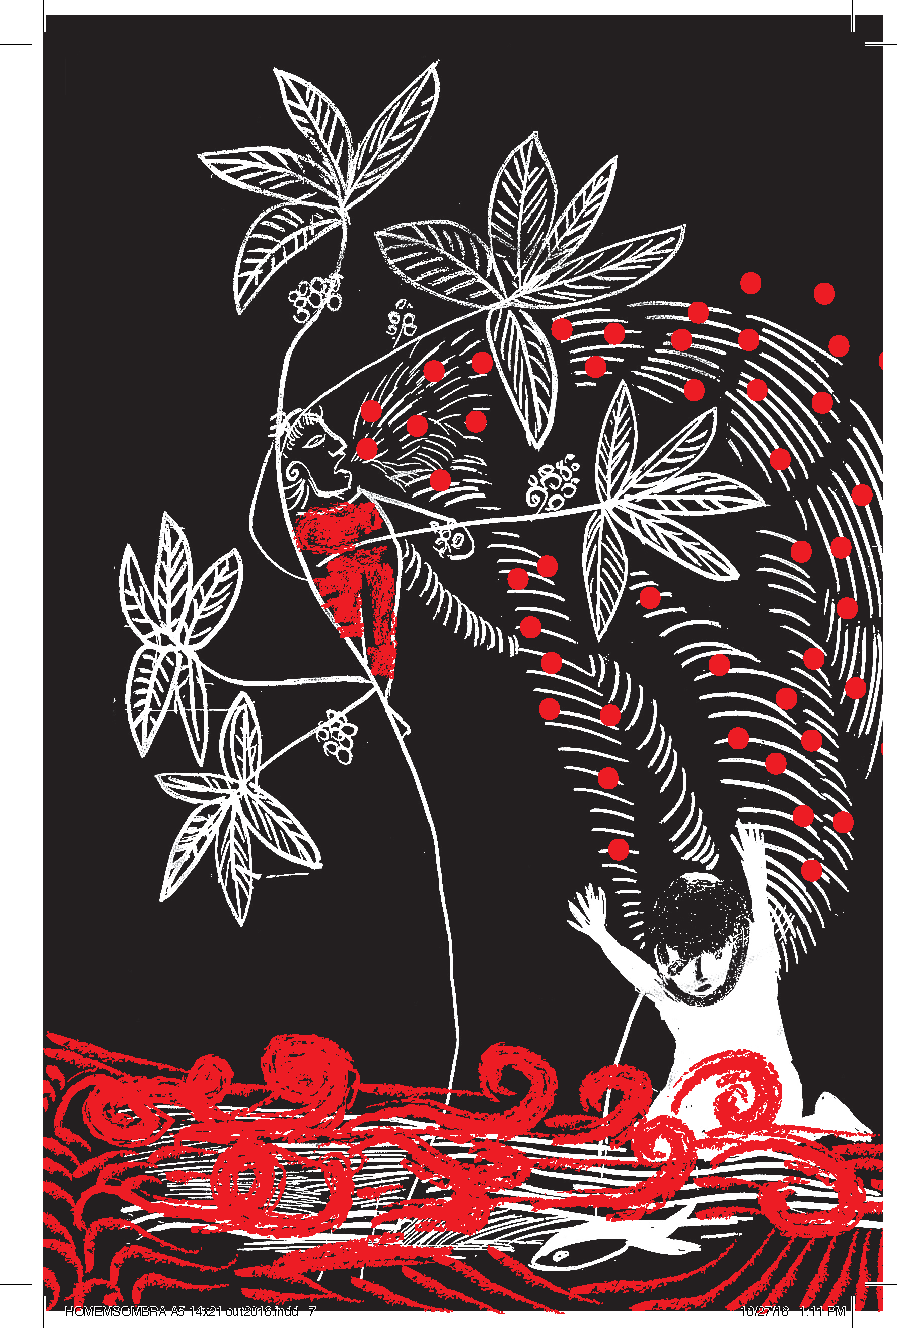
\includegraphics[width=153mm]{./imgs/img2.pdf}
\end{textblock*}

\chapter*{}

\mbox{}\vspace*{\fill}

\letra{D}{izem} que o Way Naku ficou
cantando e colhendo cucura
por muito tempo. O homem-sombra
ia de galho em galho
cantando e pegando os cachos
da fruta. Muitos dos cantos
que nós Hupd’äh cantamos nas
festas foram cantados pelo Way
Naku: o \textit{Canto do Cutia}, o \textit{Canto
Grande}, o \textit{Canto do Umarí}, o
\textit{Canto da Gente-Sombra}.

\vspace{2em}

\letra{B}{ɨ̗ g!} mah tih yamah. Sã̗p nowot
pɨd, sã̗p nowot pɨd, pɨ̗g tëgët
tɨh noh k’ët kötöh, yamap ɨhɨh,
batɨ̗b’ih. \textit{Mèt Yam}, \textit{Yam Pög}, \textit{Pej
D’áp Yam}, \textit{Batɨ̗b’ Yam}, yám nihũ̗’
mah tɨ̗ h yamah!

\vspace*{\fill}

\pagebreak

\begin{textblock*}{8in}(0pt,0pt)%
\vspace*{-2.8cm}
\hspace*{-3.2cm}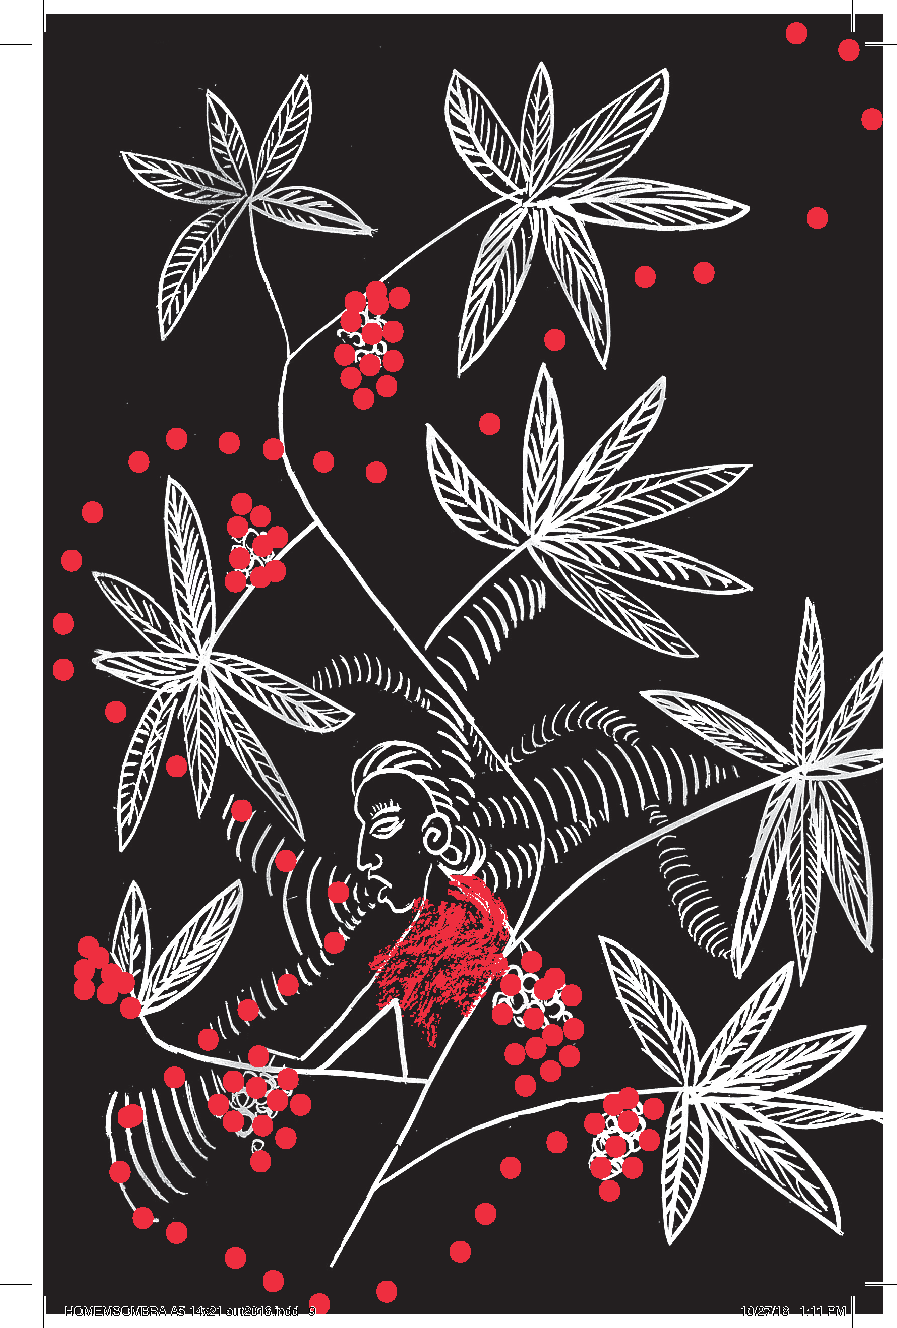
\includegraphics[width=153mm]{./imgs/img3.pdf}
\end{textblock*}

\chapter*{}

\mbox{}\vspace*{\fill}

\letra{O}{} homem hup ficou
lá a noite toda e,
depois, o outro dia
inteiro. Escutou e
prendeu os cantos
do homem-sombra.

\vspace{2em}

\letra{H}{iwag} yɨ’ɨy mah,
d’ú’ tɨh yam d’ö’öp\ldots{}

\vspace*{\fill}

\pagebreak

\begin{textblock*}{8in}(0pt,0pt)%
\vspace*{-2.8cm}
\hspace*{-3cm}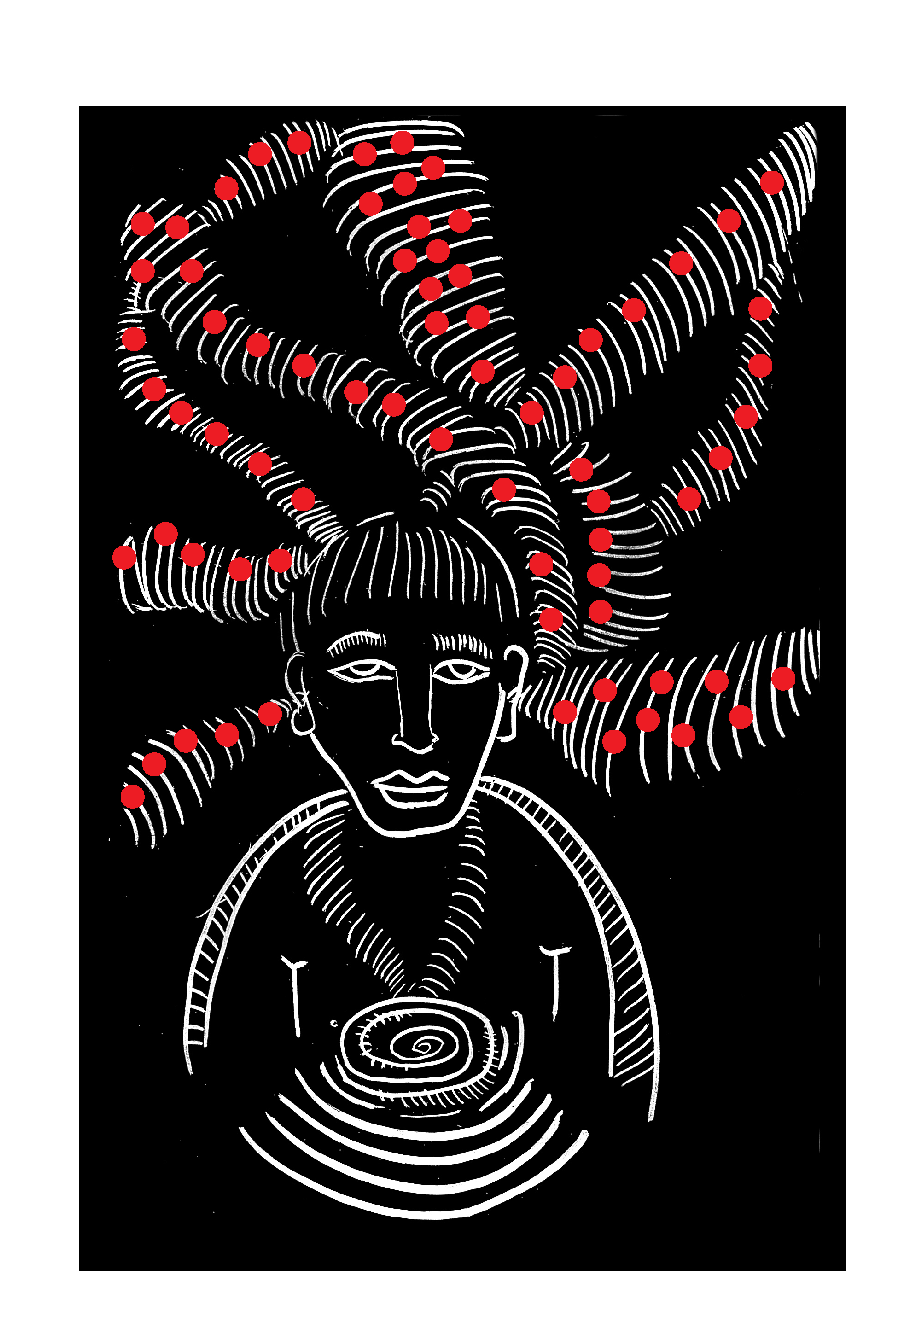
\includegraphics[width=148mm]{./imgs/img4.pdf}
\end{textblock*}

\chapter*{}

\mbox{}\vspace*{\fill}

\letra{Q}{uando} o sol
começou a nascer,
o homem hup bateu
com o terçado no
tronco da árvore
de cucura.

\vspace{2em}

\letra{H}{iwag} yɨ’ɨy, wag
hiyèt mah tɨh kɨt
hik’ëtayah, tɨh
të̖gët, pɨ̗ g tëgët.

\vspace*{\fill}

\pagebreak

\begin{textblock*}{8in}(0pt,0pt)%
\vspace*{-2.8cm}
\hspace*{-3.2cm}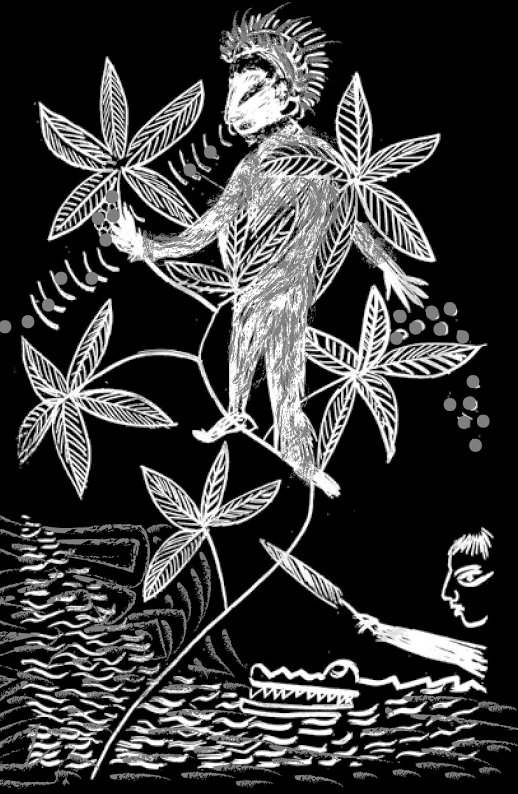
\includegraphics[width=153mm]{./imgs/img5.pdf}
\end{textblock*}

\chapter*{}

\mbox{}\vspace*{\fill}

\letra{T}{ac!} Foi o barulhão
que fez. Assustado,
o Way Naku caiu da
árvore. \textit{Puffff}!
Com medo, o homem
hup foi embora
correndo, bem
rápido! \textit{Vrummm}!

\vspace{2em}

\letra{T}{äk!} nomɨ’, yuway
mah tɨh kädhiayah.
\textit{Pë’}! Yuway mah
húp to’oh kädham
yɨ’ayah! \textit{Mmmm’}!

\vspace*{\fill}

\pagebreak

\begin{textblock*}{8in}(0pt,0pt)%
\vspace*{-2.8cm}
\hspace*{-3.2cm}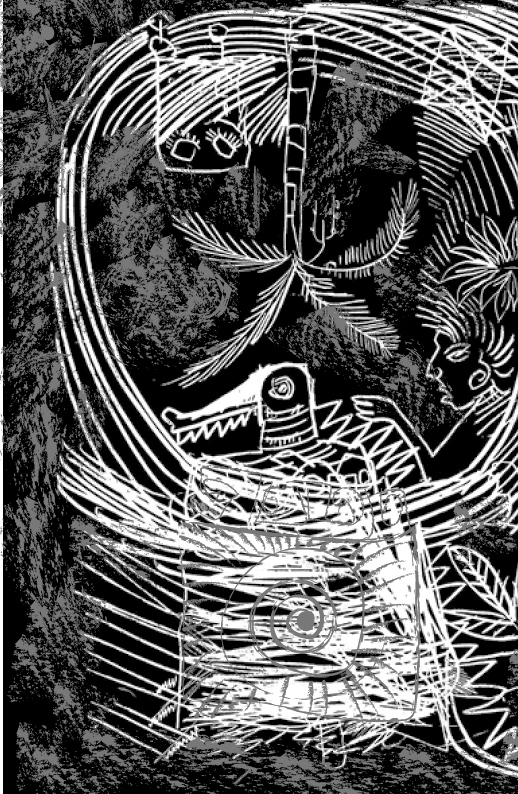
\includegraphics[width=153mm]{./imgs/img6.pdf}
\end{textblock*}

\chapter*{}

%\mbox{}\vspace*{\fill}

\letra{E}{ntão,} o Way Naku viu um
jacaré que estava deitado
na beira do rio. Pensou
que fosse o homem hup e
tentou pegá-lo. Fugindo,
o jacaré caiu na água,
\textit{tchibum}! O Way Naku,
que já estava na água,
foi atrás do jacaré. O
homem-sombra colocou a
mão na água para ver se
encontrava o jacaré.

\medskip

De repente, o jacaré deu uma\\
mordida no braço do\\
homem-sombra.

\vspace{2em}

\letra{Y}{ɨt} mah hàt yetníh. Yɨt
mah hàt noh tu’uh, \textit{tapuh}!
Yɨt mah tɨhɨt yɨ’ batɨ̗b’ noh
tu’ won kädd’öböh. Yɨt
mah hàtan tɨh d’ö’ yɨ’ɨh,
pëpë’ d’ö’ yɨ’ɨy.

\medskip

Yɨt mah tɨhan tɨh k’äç d’ö’\\
pög b’ayah, hàt b’ayah,\\
tɨnɨh mumùy súm,\\
batɨ̗b’anah.

\vspace*{\fill}

\pagebreak

\begin{textblock*}{8in}(0pt,0pt)%
\vspace*{-2.8cm}
\hspace*{-3.2cm}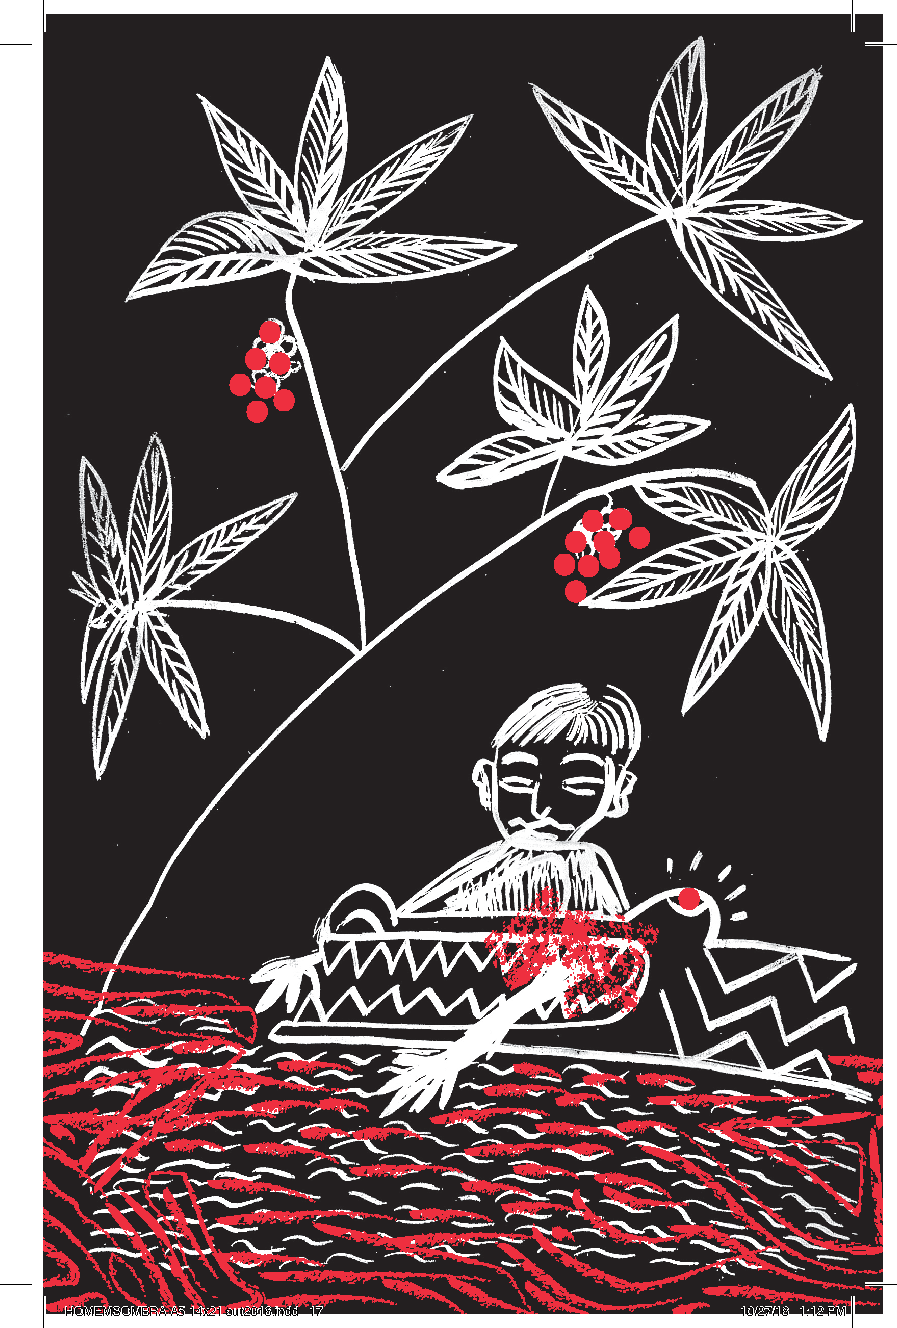
\includegraphics[width=153mm]{./imgs/img7.pdf}
\end{textblock*}

\chapter*{}

\mbox{}\vspace*{\fill}

\letra{E}{} foi assim que
o homem hup
conseguiu fugir e
voltar para casa.

\medskip

Esse foi o primeiro homem hup\\
que soube cantar os \textit{caapivaiá},\\
os cantos das festas.

\vspace{2em}

\letra{T}{ɨhɨp} húpup ham
yɨ’ay mah kah, yë
yɨ’ay mah.

\medskip

Yup ĩh mah yup, yám\\
d’ö’ hib’ahayah.

\vspace*{\fill}

\pagebreak

\begin{textblock*}{8in}(0pt,0pt)%
\vspace*{-2.8cm}
\hspace*{-3.2cm}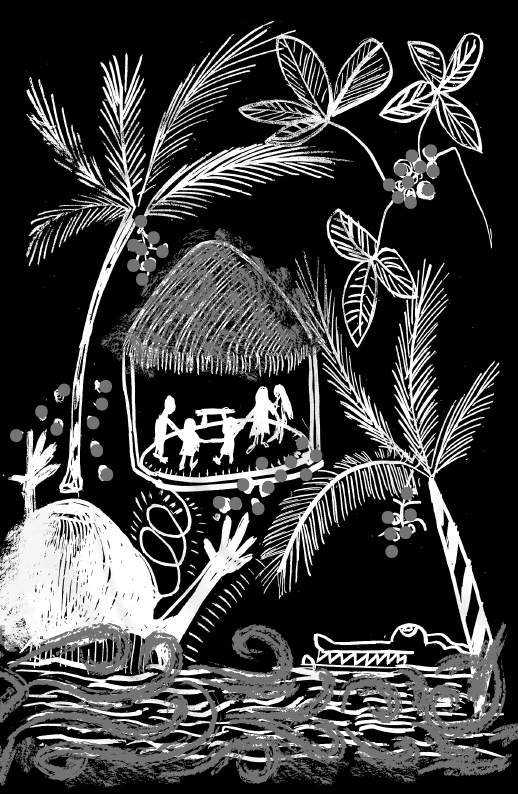
\includegraphics[width=153mm]{./imgs/img8.pdf}
\end{textblock*}

\chapter*{}

\mbox{}\vspace*{\fill}

\letra{E}{le} ouviu o homem-sombra cantar,
aprendeu bem e
começou a ensinar
para seus filhos,
irmãos, cunhados.
E até hoje todos
cantam e dançam os
\textit{caapivaiá} que animam
nossas festas.

\medskip

Foi isso o que ouvi de
meus avós.

\vspace{2em}

\letra{B}{atɨ̗b’} tɨh yamawan
wɨ’yö’ay mah, yup húp
yamayah. Yup hɨd yam
tëg n’ɨhayah. Húpd’äh
hɨd yam tëgayah.

\medskip

Ya’ap meh yɨ’ ãh wɨ’ɨh.

\vspace*{\fill}

\pagebreak

\begin{textblock*}{8in}(0pt,0pt)%
\vspace*{-2.8cm}
\hspace*{-3.2cm}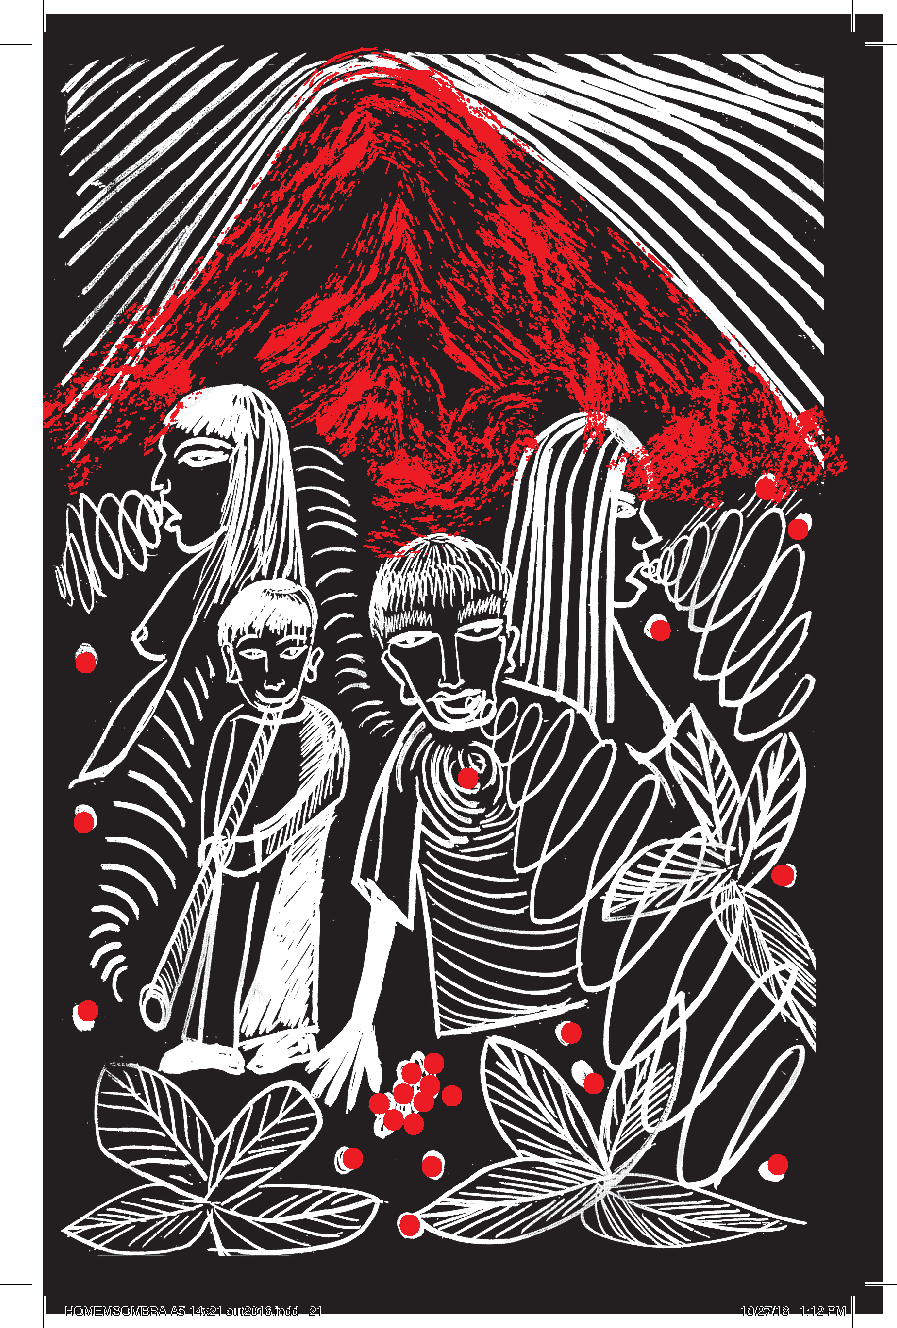
\includegraphics[width=153mm]{./imgs/img9.pdf}
\end{textblock*}

\endgroup

\chapter{Um canto do homem-sombra}

%\begin{verse}
\letra{O}{utro} galho de cucura\\
Outro galho de cucura\\
Eu jogo para baixo

\bigskip

\noindent Outro galho de cucura\\
Eu jogo para baixo\\
Colho o cacho de cucura\\
Eu jogo para baixo

\bigskip

\noindent \textit{Way Naku, yari nóóy mah\\
Marika, Way Naku}
%\end{verse}

\chapter{Way Naku}

%\begin{verse}
\letra{S}{ã̗p} nowot pɨ̗ g\\
Sã̗p nowot pɨ̗ g\\
Ãh d’äräh hitëh

\bigskip

\noindent Sã̗p nowot pɨ̗ g\\
Ãh d’äräh hitëh\\
Öy d’ö’ yö’ pɨ̗ g\\
Ãh d’äräh hitëh

\bigskip

\noindent \textit{Way Naku, yari nóóy mah\\
Marika, Way Naku}
%\end{verse}


